\documentclass[review]{elsarticle}

\usepackage{lineno,hyperref,amsmath,amsfonts,subcaption}
\modulolinenumbers[5]

\journal{Spatial Statistics}

%%%%%%%%%%%%%%%%%%%%%%%
%% Elsevier bibliography styles
%%%%%%%%%%%%%%%%%%%%%%%
%% To change the style, put a % in front of the second line of the current style and
%% remove the % from the second line of the style you would like to use.
%%%%%%%%%%%%%%%%%%%%%%%

%% Numbered
%\bibliographystyle{model1-num-names}

%% Numbered without titles
%\bibliographystyle{model1a-num-names}

%% Harvard
\bibliographystyle{model2-names.bst}\biboptions{authoryear}

%% Vancouver numbered
%\usepackage{numcompress}\bibliographystyle{model3-num-names}

%% Vancouver name/year
%\usepackage{numcompress}\bibliographystyle{model4-names}\biboptions{authoryear}

%% APA style
%\bibliographystyle{model5-names}\biboptions{authoryear}

%% AMA style
%\usepackage{numcompress}\bibliographystyle{model6-num-names}

%% `Elsevier LaTeX' style
%\bibliographystyle{elsarticle-num}
%%%%%%%%%%%%%%%%%%%%%%%

\begin{document}

\begin{frontmatter}

\title{Log-Gaussian Cox processes and sampling paths: towards optimal design}

%% Group authors per affiliation:
\author[msuaddr]{Kenneth Flagg\corref{mycorrespondingauthor}}
\cortext[mycorrespondingauthor]{Corresponding author}
\ead{kenneth.flagg@montana.edu}

\author[msuaddr]{John Borkowski}
\author[msuaddr]{Andrew Hoegh}

\address[msuaddr]{Department of Mathematical Sciences, Montana State University, Bozeman, MT 59717}

\begin{abstract}

\paragraph{Goal of this paper (placeholder abstract---add some results when
available)} Evaluate a wide variety of path designs in terms design-based
heuristics and model-based criteria for spatial prediction using Bayesian LGCP
models. Identify promising path designs. Illuminate any relationships among
design characteristics and predictive criteria that will be helpful for
constrained optimization.

\end{abstract}

\begin{keyword}
log-Gaussian Cox process\sep optimal sampling\sep model-based design\sep spatial sampling design
%\MSC[2010] 00-01\sep  99-00
\end{keyword}

\end{frontmatter}

\linenumbers

% Can name paragraphs with \paragraph{Title}


\section{Introduction}
% State the objectives of the work and provide an adequate background, avoiding a detailed literature survey or a summary of the results.

Spatial point process models have long been considered generally infeasible
because of their computational demands, but recent advances in Bayesian
computing have made the Log-Gaussian Cox process an attainable model in
practice~\citep{rueetal, lindgrenetal, illianetal, simpsonetal}. In some
applications, the entire point pattern is not fully observed due to variable
sampling effort. This is referred to as a degraded point
pattern~\citep{chakrabortyetal} and it is relatively simple to accomodate
variable sampling effort in these models using modern Bayesian computing
tools~\citep{yuanetal}. However, the literature on optimal sampling for spatial
point process models is in its infancy~\citep{liuvanhatalo}. In this article,
we present a variety of sampling path designs and assess their optimality for
LGCP models.

Point pattern data are routinely collected in species distribution studies and
ordnance response projects. These applications may use quadrat sampling or
line-transect sampling, with transect sampling being more common. When the
objective is mapping where events occur in space, various spatial mapping
procedures have been used. Traditionally these have involved aggregating the
data to grid cell counts or computing moving averages. Aggregation has the
downside of introducing arbitrary structure into the data by the choice of
gridding scheme or averaging window, and requires uneccessary computation
effort~\citep{simpsonetal}. Software is now available to fit spatial point
process models to data acquired via distance sampling and simultaneously
estimate the detection function~\citep{dspat,baser}.
% Recent example of aggregation: https://link-springer-com.proxybz.lib.montana.edu/content/pdf/10.1007/s13253-020-00386-3.pdf

In ecological settings, sampling plans are often designed around the goal of
estimating total abundance. Ordnance response surveys are typically designed
with the objective of detecting (but not necessarily mapping) intensity
hotspots~\citep{em200-1-15,flaggetal}. However, to our knowledge, there has
been very little work done in deciding where to collect data when the goal is
to map the intensity using a spatial point process model. In this paper, we
compare a variety of path design schemes with respect to a suite of
model-based and design-based criteria for simulated point pattern data.


\subsection{Spatial design}

\paragraph{Design-based sampling}
Most classical sampling work has been done for points or small quadrats
approximated as points,  rather than paths. Space-filling criteria may be good
starting points~\citep{borkowskipiepel}. Latin hypercube sampling has
space-filling properties~\cite{mckayetal,husslageetal}.

\paragraph{Space-filling curves}
Used in design of dense or stretchable circuits~\citep{ogorzalek,mazhang} and
high-dimensional data visualization in bioinformatics~\citep{hilbertvis}. Peano
curve is very flexible for filling irregular shapes~\citep{fanetal}.

Space-filling curves are one-dimensional paths constructed iteratively; as the
number of iterations goes to infinity, the limiting path has nonzero area and
actually fills the space~\citep{sagan}. For applications we stop after a finite
number of iterations. The Hilbert curve is fast and simple to construct.

\paragraph{Model-based spatial design}
Regularity is optimal for spatial prediction but randomness and a variety of
interpoint distances are best for parameter estimation~\citep{diggle}.
Inhibitory plus close pairs is a good compromise~\citep{chipetaetal2017}.


\subsection{Paths as sampling designs}

While some ideas about the characteristics of a good point design apply to
paths, creating an optimal path design is not as simple as connecting the
points of a point design with line segments. There are many ways to connect
points into a path, so optimal design criteria must apply to the whole path and
not only to the waypoints.

\citet{pollard} adaptively zigzagged their line transects in a species
abundance survey.

The Visual Sample Plan software includes features to create systamatic transect
plans and augment plans with additional transects in regions lacking spatial
coverage~\citep{vspguide}. It helps the user choose the transect spacing to
maximize the probability of detecting the presence of a hotspot of specified
size and intensity. However, it does not employ criteria to optimize spatial
prediction.

\citet{liuvanhatalo} used narrow quadrats (swaths along line-transects) as
their sampling units. The transects were short relative to the size of the
study region and not connected into a path.


%\subsection{Multi-objective optimization}

%summarize \citet{lark} and related

%we can use a large suite of criteria to explore the relationships among them

% (Don't need for this paper.)


\section{Materials and methods}
% Provide sufficient details to allow the work to be reproduced by an independent researcher. Methods that are already published should be summarized, and indicated by a reference. If quoting directly from a previously published method, use quotation marks and also cite the source. Any modifications to existing methods should also be described.

%Kenny's heuristics of a good path design:
%\begin{itemize}
%\item Should start with a sparse design with regular spacing, then refine with
%infill
%\begin{itemize}
%\item Provides good spatial coverage even if aborted early
%\item Imagine downloading a high-resolution intensity jpeg over 56k
%\end{itemize}
%\item Path should avoid sharp turns but is allowed to cross itself
%\item One option is to generate two segments at a time, first a short-to-medium
%length segment to get to the start of the next transect, then a  medium-to-long
%segment for the transect
%\item Could have new segment length be negatively correlated with the previous
%segment length
%\end{itemize}

% Andy's words:
With an eye toward practical considerations of data collection, we present
criteria to compare sampling strategies that impact LGCP estimates. We compare
plans with fixed path lengths that avoid sharp turns. Data collection equipment
(e.g. metal detectors) may have limited mobility, requiring minimizing the
number or angle of turns. The criteria that we evaluate are mean squared
prediction error (MSPE) and posterior prediction variance of the Gaussian
process.


\subsection{Sampling schemes}

{\it These are the focus, move them earlier?}

\subsubsection{Parallel line transects}

Parallel straight-line transects are common in ordnance response studies and in
ecological studies using distance sampling. Systematic designs are common
because they provide good spatial coverage in the sense that any point in the
study region has a known maximum distance from the path. For point designs,
systematic designs are optimal for prediction, simple random samples are
optimal for estimation, and inhibitory with close pair designs are becomming a
popular compromise. We adapt all of these to the parallel line transect
setting. We use line transects running north-south, with three ways of choosing
the horizontal coordinate: simple random sample (SRS), systematic with a random
starting point and even spacing, inhibitory plus close pairs.
Figure~\ref{linexsects} shows an example of each scheme with 25 transects.

For the inhibitory plus close pairs, we vary the numbers of paired and unpaired
transects. The total number of transects is 10, 25, 50, or 70, with 10\% and
20\% of the transects (rounded to the nearest integer) as redundant members of
a pair. The remaining primary transects were placed according to a
one-dimensional Strauss process with \(\gamma = 0.05\) and a radius of 80. Then
each redundant transect was randomly paired to a primary transect, an placed
within an 80 unit radius of the primary transect according to a uniform
distribution.

We should note that our we will be using an isotropic covariance function in
the model. If an anisotropic model is used, parallel transects may need to be
augmented with perpendicular transects so that the observed data provide the
full range of pairwise distances in other directions.

\begin{figure}
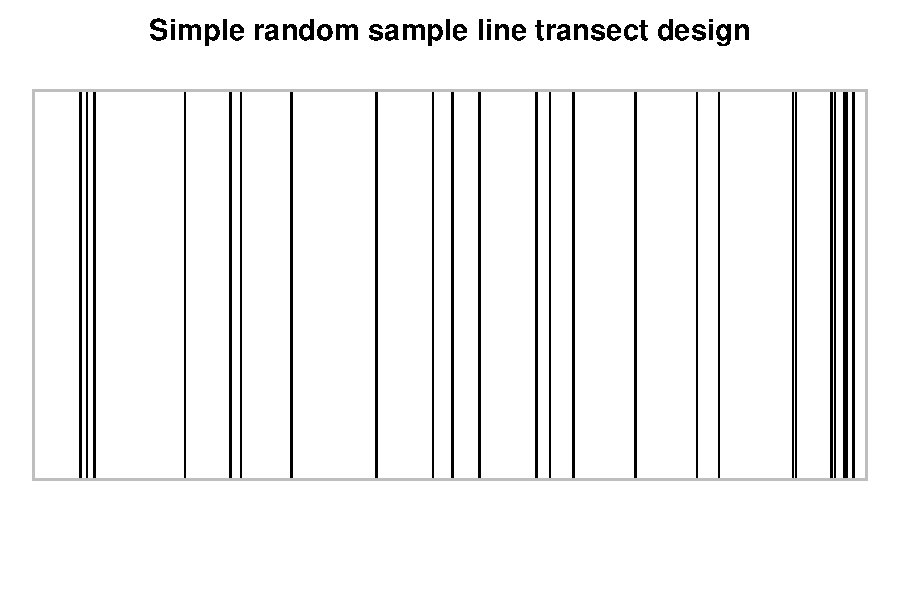
\includegraphics[width=5in]{SRS000176.pdf}

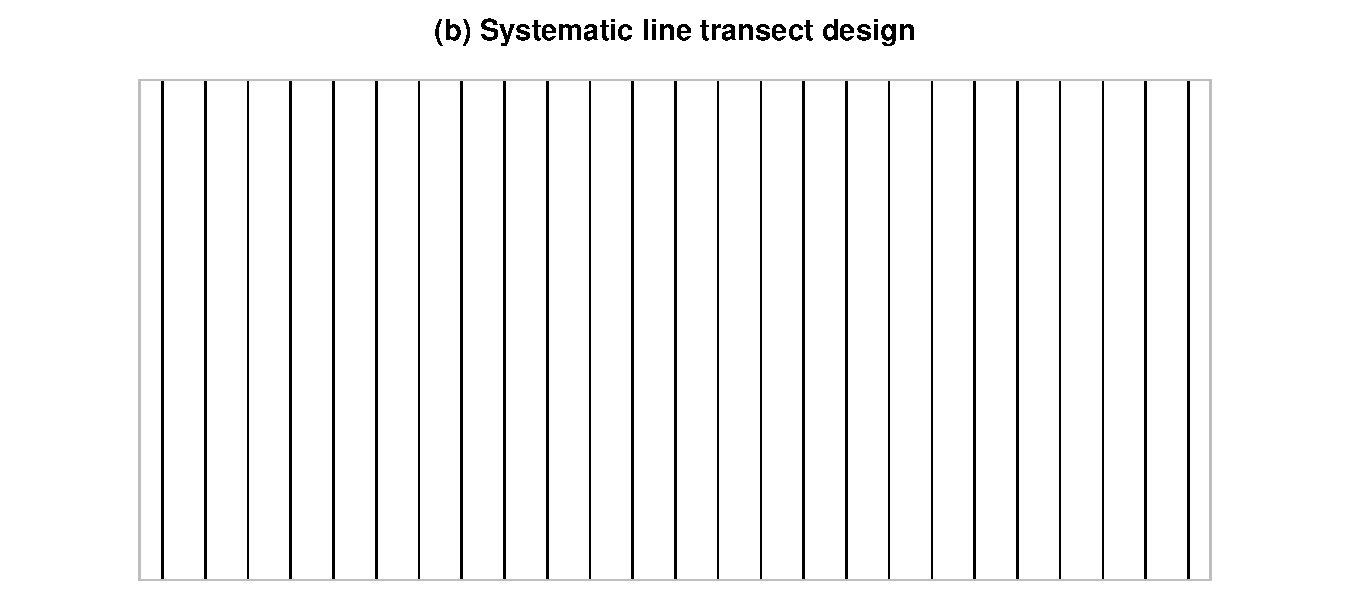
\includegraphics[width=5in]{Sys000141.pdf}

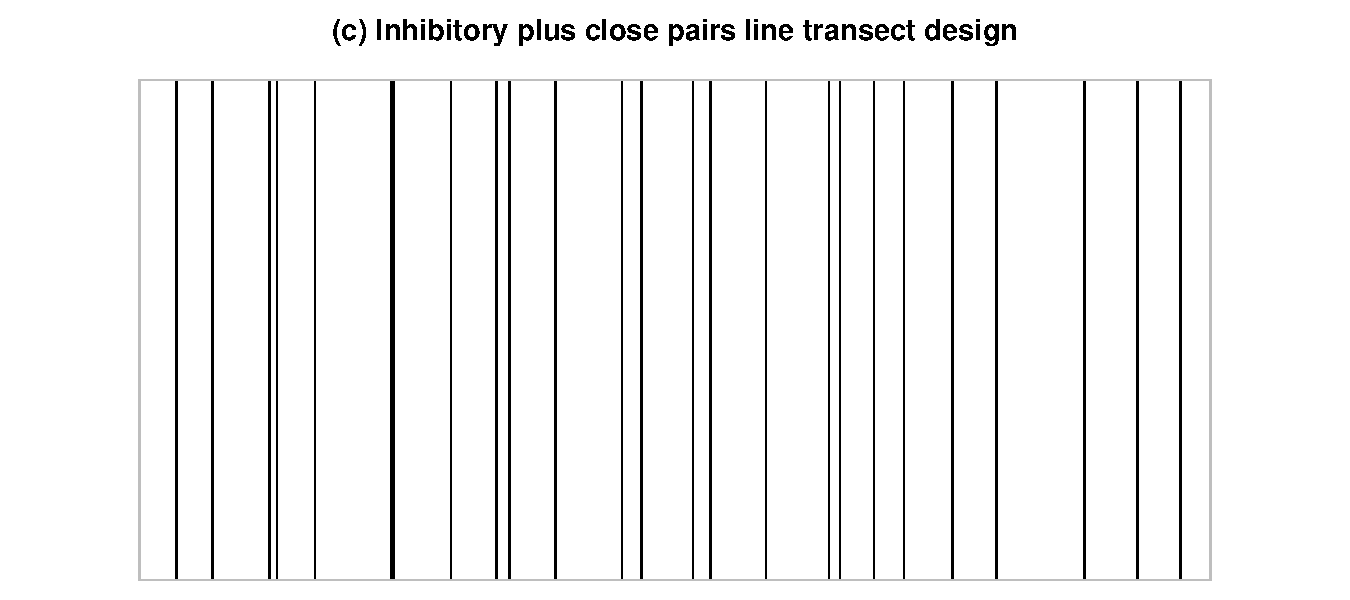
\includegraphics[width=5in]{Inhib000171.pdf}

\caption{Examples of three different parallel line transect designs with the
same number of transects.}
\label{linexsects}
\end{figure}

\subsubsection{Parallel serpentine transects}

One simple way to observe a greater variety of locations and different
directions is to add lateral zigzags to transects. We include alternate right
and left turns at right angles to create serpentine transects. This could
decrease prediction variance because many points in the study area will be
closer to the path than they would be under a similar plan of line transects.
{\it (Check the math---is this true? And does similar mean same length or same
number of transects?)} They will also improve estimation of covariance
parameters in the presence of anisotropy.

We generate designs with 7, 22, 47, and 67 serpentine transects. We vary the
complexity of the serpentines by using versions with 5 and 8 zigzags. We define
a zigzag as a single north-south segment or a pair of connected north-south and
east-west segments. The lengths of the east-west segments are set so that the
total distance equals the total distance of a line transect design with
three more transects. Figure~\ref{serps} shows examples.

% What to do with the comments about anisotropy? Consolidate them and put them
% in one spot? Anisotropic models are rarely used (underused) and we are
% simulating from isotropic models, but "go in more than one direction if you
% have anisotropic data" is advice worth spending a paragraph on.

\begin{figure}
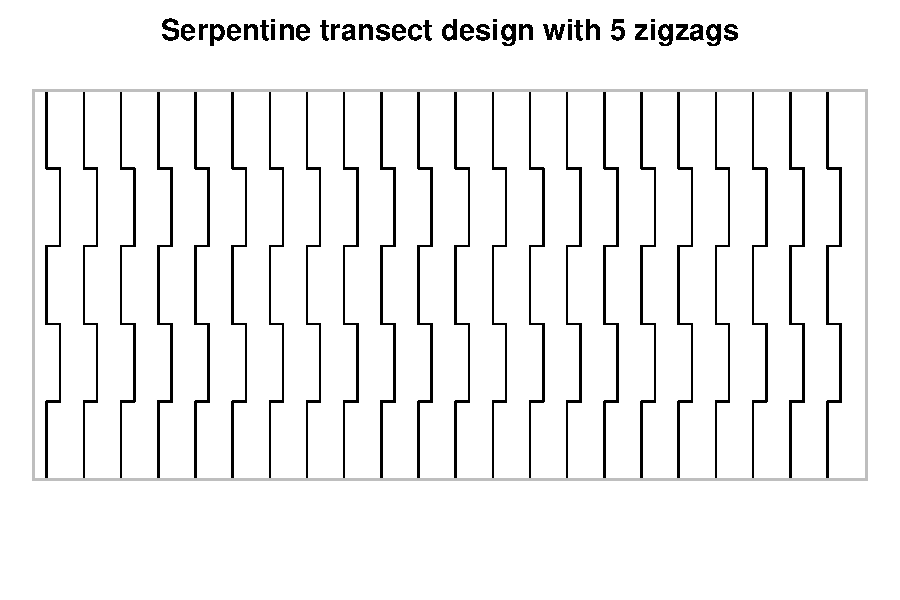
\includegraphics[width=5in]{Serp000124.pdf}

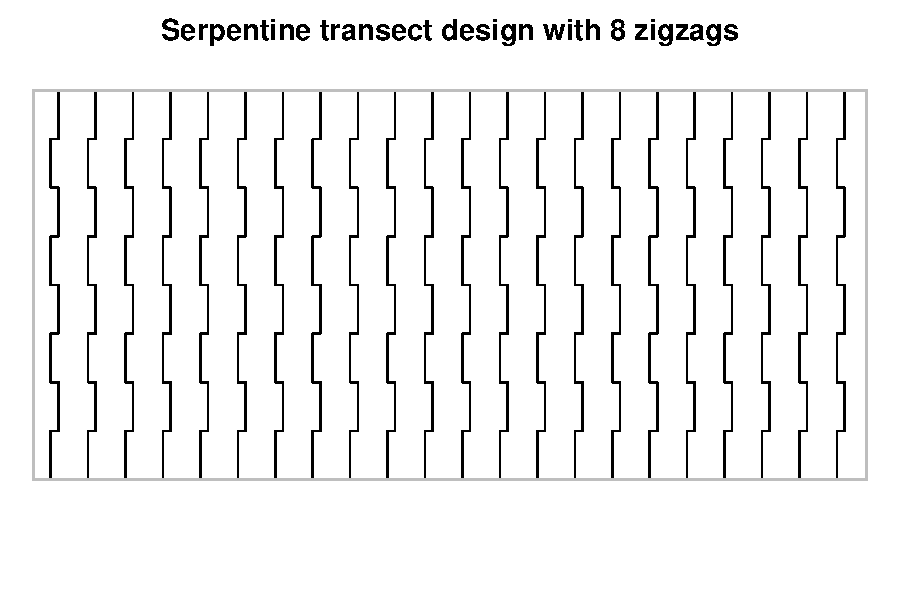
\includegraphics[width=5in]{Serp000539.pdf}

\caption{Examples of systematic serpentine transect designs of the same
distance. The number of zigzags is the number of north-south segmetns per
transect.}
\label{serps}
\end{figure}

\subsubsection{Latin hypercube sampling}
Random Latin hypercube sampling (LHS) produces a design that spreads discrete
points through a (potentially high-dimensional) design space, ensuring that
the full range of each dimension is included while remaining balanced and
keeping the number of points small. This is done by partitioning each dimension
into a specified number \(k\) of intervals (thus stratifying the design space
into \(k^{d}\) cells), selecting a Latin hypercube design to determine which
cells will contain a design point, and then drawing each design point from a
uniform distribution over its cell. In two dimensions, this scheme produces
point designs with good spatial coverage properties. We use the LHS design as
waypoints for a path. Because distance is typically a criterion to be
minimized, we treat this as a traveling salesperson problem (TSP) and use the
shortest path through the waypoints as our design. This LHS-TSP scheme produces
paths that have many sharp corners but leaves few large voids (example in
Figure~\ref{lhstsp000161}). A downside of this design scheme is that the length
cannot be specified directly, and only certain distances are possible depending
on the number of bins used. We use designs with \(k\) = 50, 300, 1200,
and 2400 bins. Waypoints are generated by the \texttt{lhs} R package~\cite{lhs}
and connected into a the shortest path by the \texttt{TSP} package~\citep{tsp}.

\begin{figure}
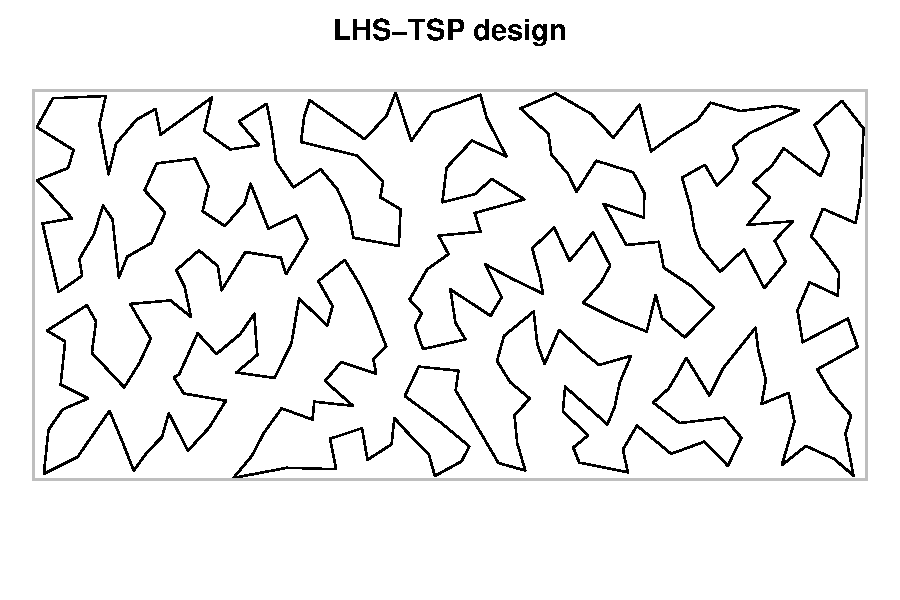
\includegraphics[width=5in]{LHS-TSP000161.pdf}
\caption{Example of a shortest path through a Latin hypercube sampling design.}
\label{lhstsp000161}
\end{figure}

\subsubsection{Space-filling curves}
Hilbert curve generated by HilbertVis package~\citep{hilbertvis}. This is a
deterministic design, so a random offset is added.

\begin{figure}
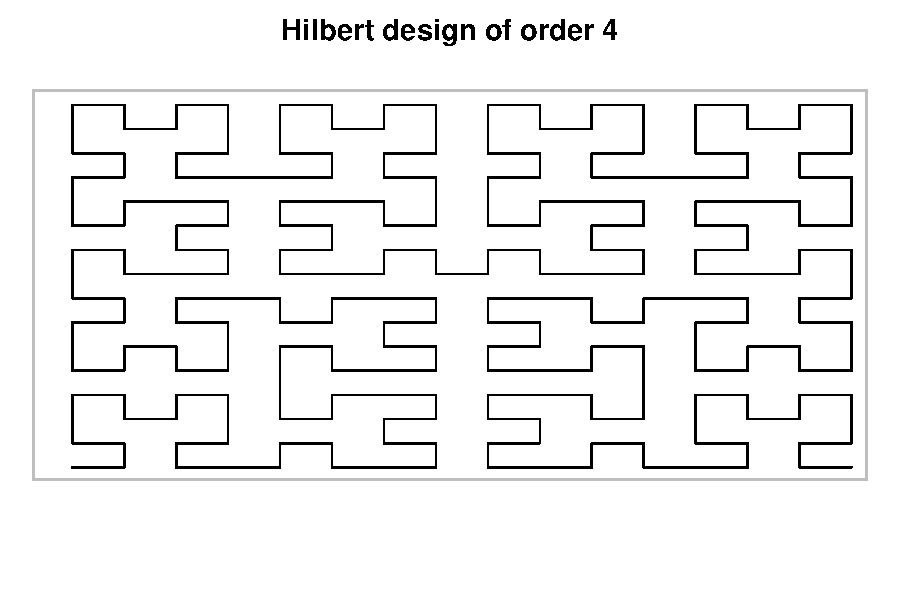
\includegraphics[width=5in]{Hilbert000180.pdf}
\caption{Example of a Hilbert curve design.}
\label{hilbert000180}
\end{figure}

%\paragraph{Particle movement model}
%Models the way data are actually collected. Waypoints generated sequentially by
%generating a jump distance and a direction. The jump distance is generated from
%a scaled beta distribution, and negatively correlated with previous jump
%distance. This behavior should approximately alternate between a short
%``transition'' and a long transect. The negative correlation was achieved by
%applying a \(1 - x\) transformation to a beta autoregressive
%process~\citep{mckenzie}. The direction angle is drawn from a bimodal
%distribution that is symmetric around 0 (a normal distribution reflectd about
%0). {\it explain the Strauss part}

%{\it set up to think about adaptive sampling (adding a transect at a time or
%stopping early but don't actually do it here)}

%\begin{figure}
%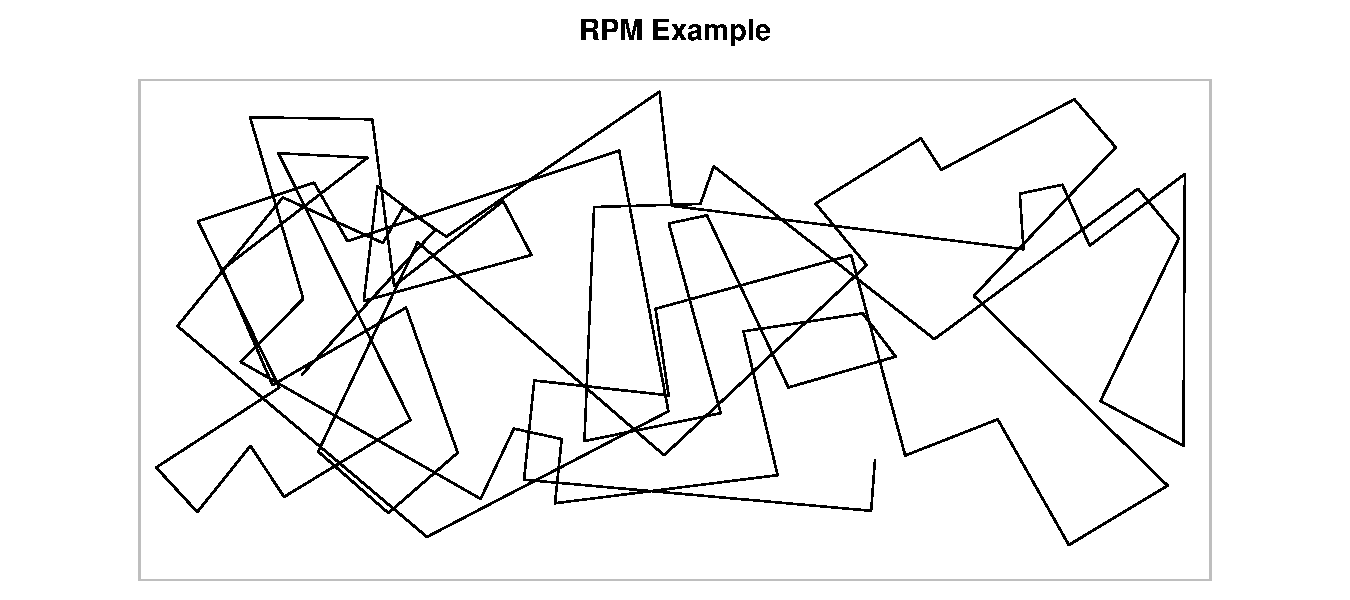
\includegraphics[width=5in]{RPM001107.pdf}
%\caption{Example of a random particle movement design.}
%\label{rpm001107}
%\end{figure}


\subsection{Model fitting}

INLA~\citep{rueetal}, SPDE~\citep{lindgrenetal}, off-grid~\citep{simpsonetal},
Flagg and Hoegh (2020) \emph{knock on wood}


\section{Simulation Study}

We consider a fictitious site \(\mathcal{R}\) with the simple shape of a 1500
unit by 700 unit rectangle. In this site, we will simulate two data generating
models meant to produce random intensity functions with with hotspots. First,
a LGCP with latent GP mean \(\mu = \log(250 / |\mathcal{R}|)\) and a
Mat\'{e}rn covariance with \(\nu = 1\), \(\sigma = 2\), and
\(\text{range} = 200\). This model produces relatively unstructured hotspots
due to large variability in the GP.

Second, the superposition of a two-stage cluster process superposed and a
LGCP. The cluster process (a Neyman-Scott or, more specifically, a Thomas
process) is constructed as follows. The number of clusters is Poisson with
mean 3. The number of events per cluster is Poisson with mean 200. The cluster
centers distributed uniformly over \(\mathcal{R}\). Events come from a
bivariate normal distribution with mean equal to the cluster center and
variance \(\boldsymbol{\Sigma} = \tau^{2}\mathbf{I}\), \(\tau = 50\). The LGCP
has \(\mu = \log(250 / |\mathcal{R}|)\) and Mat\'{e}rn covariance with
\(\nu = 1\), \(\sigma = 1\), and \(\text{range} = 200\). This model is based
upon the typical conceptual model of a firing range, with a background process
(represented by the LGCP) and a small number of higher-intensity foreground
clusters containing the events of interest.

Path design schemes:
\begin{itemize}
\item Simple random sample of north-south line transects
\begin{itemize}
\item \(\text{Number of transects} = 10, 25, 50, 70\)
\item Expect high variance, large prediction error in big gaps.
\end{itemize}
\item Systematic sample of north-south line transects
\begin{itemize}
\item \(\text{Number of transects} = 10, 25, 50, 70\)
\item Uniformly distributed starting point
\item Constant spacing
\item Expect low bias and ok variance, can miss structures at certain sizes,
may not have best space-filling properties.
\end{itemize}
\item Systematic sample of north-south serpentine transects
\begin{itemize}
\item \(\text{Number of transects} = 7, 22, 47, 67\)
\item Uniformly distributed starting point
\item Constant spacing
\item \(\text{Number of zigzags} = 5, 8\)
\item Horizontal zigzag distance set so that the total horizontal distance
traveled equals 2100 units (the length of 3 non-zigzag line transects)
\item Expect better space-filling properties than line-transect designs,
lower bias/variance farther from path, would be better at estimating
anisotropic covariance than line-transects.
\end{itemize}
\item Inhibitory plus close pairs sample of north-south line transects
\begin{itemize}
\item \(\text{Total number of transects (including pairs)} = 10, 25, 50, 70\)
\item \(\text{Number of pairs} = 0.1, 0.2\) times the total number of transects
(rounded up or down to nearest whole number)
\item Pairs uniformly distributed within radius of primaries,
\(\text{max pair radius} = 1500 / \text{total number of transects}\)
\item Position of primaries generated from a 1-dimensional Strauss process with
\(\gamma = 0.05\)
\item A compromise between SRS and systematic in every way.
\end{itemize}
\item Latin Hypercube Sampling waypoints
\begin{itemize}
\item \(\text{Number of bins} = 50, 300, 1200, 2400\)
\item Expect low bias/variance per unit distance traveled, many sharp corners,
some big open areas.
\end{itemize}
\item Hilbert curve
\begin{itemize}
\item \(\text{Order} = 3, 4, 5, 6\)
\item Created in square and then scaled to fit in \(\mathcal{R}\)
\item A uniform random offset added equal to spacing between segments
\item Expect good space filling, good bias and variance, lots of short
segments.
\end{itemize}
\end{itemize}

{\it (Probably should move explanations of schemes to appendix.)}

100 designs from each scheme. All events within a 2 unit radius of the path are
observed. Whole experiment repeated for 5 realizations from each data
generating model.

Model:

\begin{itemize}
\item \(\mathbf{X}\) is a Poisson process on \(\mathcal{R}\) with intensity
\(\lambda(u)\)
\item \(\log[\lambda(u)] = \mu + \mathbf{e}(u)\)
\item \(\mu \sim \mathrm{Unif}(-\infty, \infty)\)
% Or \(\mathrm{N}(0, \infty)\)?
\item \(\mathbf{e}\) is a Gaussian process with mean \(\mathbf{0}\) and a
Mat\'{e}rn covariance function with fixed \(\nu = 1\)
% Remember alpha = nu + d/2 so alpha = 2 and d = 2 imply nu = 1.
\item PC prior on \(\sigma\) and \(\rho\) with \(\mathrm{Pr}(\sigma > 3) = 0.1\)
and \(\mathrm{Pr}(\rho < 100) = 0.1\) \citep{fuglstadetal,simpsonpc}
\item SPDE approach of \citet{lindgrenetal} using mesh in Figure~\ref{meshfull}
\item Likelihood factorization of \citet{simpsonetal}
\end{itemize}

\begin{figure}
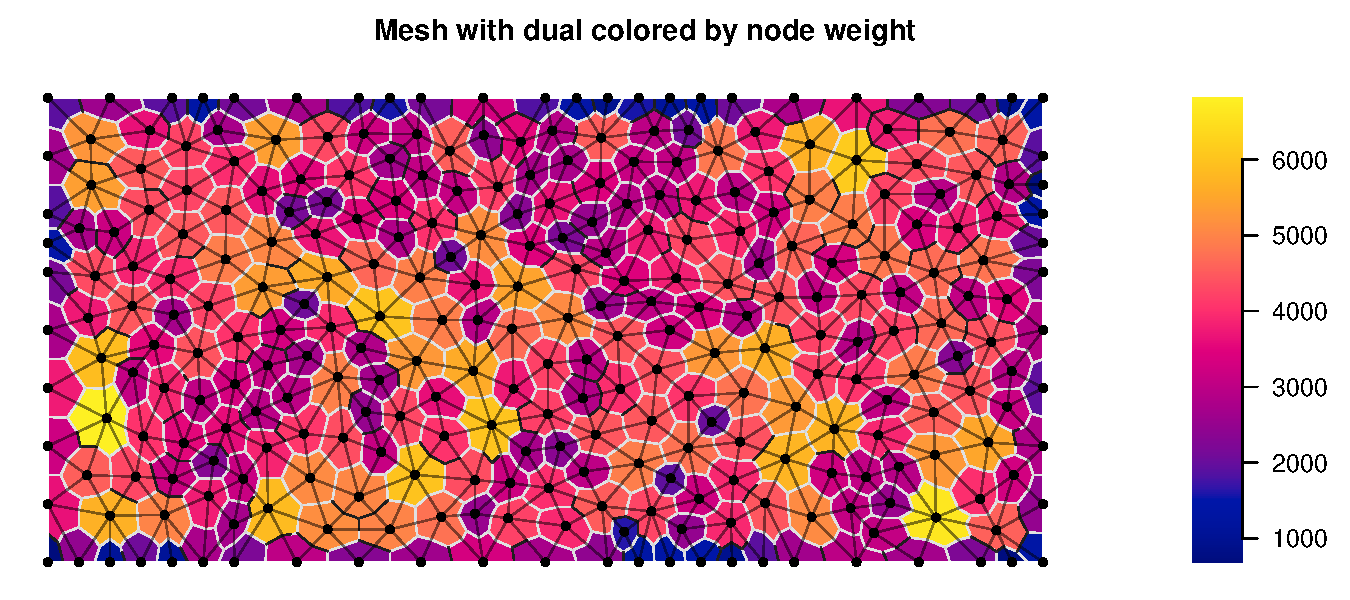
\includegraphics[width=5in]{mesh_full.pdf}
\caption{Illustration of the mesh and associated numerical integration scheme
used to approximate the latent GP.}
\label{meshfull}
\end{figure}


%\section{Theory/calculation}
% A Theory section should extend, not repeat, the background to the article already dealt with in the Introduction and lay the foundation for further work. In contrast, a Calculation section represents a practical development from a theoretical basis.


\section{Results}
% Results should be clear and concise.

look at examples of designs that minimize each criterion

look at examples of designs along the Pareto front


\section{Discussion}
% This should explore the significance of the results of the work, not repeat them. A combined Results and Discussion section is often appropriate. Avoid extensive citations and discussion of published literature.

discuss starting points for optimization and sequential design

practical issue: path will be smoothed, no instantaneous direction changes at
corners, equipment may have limitations which is why we looked at number and
distribution or turn angles

could incorporate turns into loss function or use multi-objective
optimization~\citep{lark}


\section{Conclusions}
% The main conclusions of the study may be presented in a short Conclusions section, which may stand alone or form a subsection of a Discussion or Results and Discussion section.


\appendix
\section{Notation and Terminology}

\begin{itemize}

\item process defined on \(\mathcal{D} \subset \mathbb{R}^{d}\), domain of the
intensity function, in this manuscript \(d = 2\)

\item observation window \(\mathcal{S} \subset \mathcal{D}\)

\item define three regions:
\begin{itemize}
\item the domain \(\mathcal{D}\) over which the process mathematically operates
\item the study region \(\mathcal{R}\) over which inferences are desired
\item the observed/sampled observation window \(\mathcal{S}\)
\end{itemize}

\item general relationship is \(\mathcal{S} \subset \mathcal{R}
\subset \mathcal{D} \subset \mathbb{R}^{d}\) where all of the subset symbols
taken to mean ``subset or equal''

\item \(\mathcal{D}\) can be bounded or unbounded (often equal to
\(\mathbb{R}^{d}\)), $\mathcal{S}$ practically always bounded, \(\mathcal{R}\)
bounded or unbounded depending on application and inferential goals

\item the ``fully surveyed'' (censused) situation is
\(\mathcal{S} = \mathcal{R}\)

\item survey path \(\mathcal{P}\) is a one-dimensional subset of
\(\mathcal{R}\)
\begin{itemize}
\item set of one or more sequences of waypoints connected by line segments
\item \(\mathcal{S}\) is the set of all points within a fixed (and assumed
known) radius of \(\mathcal{P}\)
\end{itemize}

\item \(\mathbf{X}\) point process on \(\mathcal{R}\), \(\mathbf{x} = \{x_{1},
\dots, x_{n}\}\) realized point pattern
\begin{itemize}
\item \(\mathbf{X}_{\mathcal{S}} = \mathbf{X} \cap \mathcal{S}\) the
 restriction of \(\mathbf{X}\) to \(\mathcal{S}\), \(\mathbf{x} = \mathbf{X}
\cap \mathcal{S}\) the realized observeable point pattern
\end{itemize}

\item point \(x \in \mathbf{x}\) called an event

\item intensity function \(\lambda(u)\)

\item types of ``points'' in space:
\begin{itemize}
\item \(x\) event in the point pattern
\item \(s\) numerical integration node
\item \(u\) arbitrary location in \(\mathcal{D}\) used to index intensity
function and predictors
\end{itemize}

\item \(z(u)\) a column vector of covariates/predictors at \(u\) (not used in
this manuscript)

\item ``point'' refers to a \(u\) unless clearly stated otherwise

\item bold for sets and spatial processes, normal italics for spatial vectors

\item \(y\) and variations will be used for objects derived from the point
pattern, e.g. marks, pseudodata

\item distance sampling fits into the framework with expansion of notation
to include a (nontrivial) detection function and differentiate between the
observed and observable point patterns

\end{itemize}


%\section{Extension of Nearest Neighbor Distance to Paths}


\section*{References}

\bibliography{lgcp_sampling.bib}

\end{document}
